\documentclass{btswhitepaper}
\title{BitShares Testnet Stress-test}
\author{
 Fabian~Schuh
 BitShares Europe, bitshares.eu\thanks{This work was supported by ChainSquad GmbH, BitShares-Munich and honorable members of the bitsharestalk.org community.}\\
 Erlangen (Bavaria), Germany\\
 \texttt{fabian@bitshares.eu}
}
\begin{document}
\maketitle

\begin{abstract}%
 BitShares 2.0 is an industrial-grade decentralized platform built for
 high-performance financial smart contracts. In order to show its capabilities
 in the field, we have conducted a stress test on the public testnet. The
 testnet has been deployed with the identical code base that is used for
 the BitShares network and has nodes around the globe. A multi-phase
 stress-test has been proposed and accepted that modifies the maximum
 transaction size, maximum block size and block confirmation times in the live
 network during the stress test. Validators have been kept up to date by means
 of stake-weighted voting~\cite{bts:general}.
\end{abstract}

\section    { Introduction                       } The Graphene Platform has been developed by Cryptonomex specifically for
BitShares, went through many changes and has done its best to stay on top of
blockchain technology. One of it's public forks, BitShares, is publicly traded
for over 2 years and has yet to show it's full potential. For this reasons, we
have deployed a testnet using the very same technology that BitShares is built
on, specifically for testing algorithms, implementations and also scalability.

Here, the term \emph{scalability} refers to the amount of transactions that can
be applied to the blockchain at scale. Several factors need to be taken into
account to correctly interpret any results obtained through testing. Among
these are the specification of the deployed servers (CPU/RAM) that produce the
blocks (validators), the interconnectivity of the nodes in the Peer-2-Peer
network, the round-trip times and latency between nodes, as well as the
geographical distance between nodes.

Obviously, a globally distributed network represents the worst case scenario
when it comes to latency between nodes limited mostly by the speed of light and
the size of the planet. A network that is hosted locally can result in better
overall performance but doesn't offer the same robustness and redundancy as a
global network.

The number of validators, furthermore, does not affect the throughput as long
as all active validators can keep up with the requirements of the network. All
active validators are treated equally and are given a slot to produce their
blocks in each round~\cite{bts:general}. Increasing the number of validators
(a.k.a. witnesses) comes with an increased robustness against server failures,
but also results in a longer period to reach transaction
finality~\cite{bts:general} which describes the absolute irreversibility of
transactions after 2/3 of all validators approved a given block and its'
transactions.

The goal of the public stress-test performed on the graphene-based testnet was
to identify the limiting factors and bottlenecks at scale with multiple parties
involved. We furthermore wanted to demonstrate scalability of current state of
the art blockchain technologies.
 
\section    { Testnet Setup                      } We have deployed a separated blockchain for the public testnet that has been
launcehd in January 2016. That blockchain was open to the public and every new
account has been donated some of the core assets called \texttt{TEST}. By the
time of the stress-test, the blockchain had over \num{6800000} blocks,
and over \num{25000000} operations processed.
 
\subsection { Software                           } The software for the testnet backend has been maintained by BitShares Europe and is
available for review on github.com. It is an almost identical fork of the
Graphene code base that BitShares is built on with only marginal changes to
accommodate the separated blockchain.

The tools that have been developed for the stress-test and the analysis are
mostly available in separate repositories as well.
 
\subsection { Validators                         } The validators' job is to collect unconfirmed and pending transactions as
received through a Peer-2-Peer network, verify and validate them and publish
your approval over those transactions in form of a signed block that carries
those transactions.

Given that the Graphene testnet also uses Delegated Proof of Stake (DPOS) as
it's consensus mechanism, the validators (a.k.a. block producers) can be voted
in and out by means of the stake-based governance system~\cite{bts:general}.
This allows us to 
\begin{inparaenum}
 \item modify the number of validators
 \item replace failing validators by standby validators
 \item pick validators that are closer geographically (if location is known)
\end{inparaenum}
every maintenance interval. This interval is used to tally all votes made
since the previous maintenance block and is set to \SI{5}{min} on the
test-network.

At the beginning of the stress-test, we will have these validators active:

\begin{compactdesc}
 \item[blckchnd-x] Intel Xeon E3, 32GB RAM, bare bone, Germany
 \item[blckchnd-test] Intel Xeon E3, 32GB RAM, bare bone, Germany
 \item[jim.witness1] Intel Xeon® E5, 28-56GB RAM, Azure, South Korea
 \item[smailer-5]  Intel Xeon E3, 32GB RAM, Germany
 \item[init0] Intel Core i7, 32GB RAM, bare bone, Germany
 \item[init2] Intel Core i7, 32GB RAM, bare bone, Germany
 \item[lafona2] Intel Avoton, 32GB RAM, France
 \item[delegate.ihashfury] Intel Atom C2750, 32GB RAM, bare bone, France
 \item[f0x] Intel Xeon E5, 56GB RAM, Azure, USA
 \item[alpha-jpn] Intel Xeon E5, 56GB RAM, Azure, Japan
 \item[bravo-bra] Intel Xeon E5, 56GB RAM, Azure, Brasil
 \item[charlie-usa] Intel Xeon E5, 56GB RAM, Azure, USA
 \item[delta-gbr] Intel Xeon E5, 56GB RAM, Azure, UK
 \item[rngl4b] Intel Xeon E5, 32GB RAM, bare bone, Luxembourg
 \item[taconator-witness] Intel Xeon E5, 32GB RAM, Switzerland
 \item[arthur-devling] Intel Xeon E5, 39GB RAM, France
 \item[fr-blockpay] 
 \item[de-blockpay] 
\end{compactdesc}
 
\subsection { Reference Full Node and Seed Node  } A bare bone reference node is provided by BitShares Europe that allows
participants to interface with the Peer-2-Peer network without running their
own full-nodes. The endpoint is available at
\texttt{wss://node.testnet.bitshares.eu} and is powered by a Intel Core i7 with
64GB of RAM which carries two fully balanced full nodes to deal with the
traffic.

A frontend-wallet is provided under \texttt{https://testnet.bitshares.eu}.
 
\section    { Limiting Factors                   } In this section we briefly discuss the limiting factors we have identified
prior to the stress-test. For the sake of proper description, we first need to
look into the distinction of \emph{blocks}, \emph{transactions}, and
\emph{operations}.

Similar to other blockchain technologies (i.e. Bitcoin), a single block may
contain multiple transactions. Each transaction is signed by one or multiple
entities and thus requires the validators to perform elliptic curve signature
verification as well as public key recovery for authorization.

In contrast to other blockchains, Graphene-based blockchain \emph{explicitly}
allow to bundle multiple \emph{operations} into a single transaction. Similar
to Bitcoin allowing to bundle multiple outputs, but with the options to execute
different smart contracts offered by the blockchain subsequently. The easiest
application is similar to Bitcoin's multi-send feature where a single user
sends bitcoins to many addresses. In the case of Graphene/BitShares, the user
would also sign a single transaction with a single signature but the
transaction would carry many \texttt{transfer} operations. Additionally, a
user may put a combination of \texttt{trade}/\texttt{transfer}/\texttt{borrow}
operations (or any other) into a single transaction to ensure that they are
executed subsequently.

As can be seen, the main difference between bundling many transactions into a
block and bundling many operations into a transactions is that in the latter
case, the operations are guaranteed to be executed subsequently and that only a
single authorization (e.g. signature) needs to be validated and verified.

This distinction is important as our test results will clearly distinguish
between the throughput of \emph{operations} and the throughput of
\emph{transactions}.

From a scalability point of view, the limiting factors are the time and
resources that are required to validate a signature for a given transaction and
the time and resources that are required to append a transactions to the
blockchain and execute its corresponding smart contract/operation.

Since the Graphene technology is built such that the signature validation can
be done independent of the blockchain's current database state, the signature
verification and key recovery can be trivially parallelized by means of a
cluster or the use of a graphics processing unit (GPU). However, as the
required software for this parallel verification was not available at the time
of the stress-test, we expect the throughput to be significantly higher once we
can validated on a GPU.

For this reason, and because we want to see the limiting factors when applying
validated transactions to the blockchain, parts of our test scenario are
focused around producing transactions that carry hundreds of \emph{transfer}
operations with just a single signature to be verified.

\section    { Phases of the Stress-Test          } Since we use Graphene as our underlying technology, most blockchain parameters
can be changed in real-time with no need for protocol upgrades or hard forks.

In contrast to the public BitShares network, the majority of the stake in the
public testnet is owned by BitShares Europe and allows us to change the
parameters without the need to collude with other stakeholders.

This allows us to setup a multiphase stress-test that will go through a set of
different blockchain parameters to gradually increase the amount of
processed transactions on the blockchain.
 
\subsection { Modified Blockchain Parameters     } For our stress-test, we decided to focus on three blockchain parameters only:

\paragraph{Max. block size}
This limit allowed us to modify the size of the blocks that are considered valid
by the network. For our test, the size will be between \SI{1}{MB} and
\SI{10}{MB}. The limiting factor is the supported data rate and connectivity of
the validating nodes since blocks need to be produced and broadcasted within a
certain time interval. A broadcast block needs to be received by the subsequent
validator in time, otherwise the subsequent block cannot be linked to the
expected previous block properly.

\paragraph{Max. transaction size}
Each \emph{block} can carry multiple \emph{transaction} and, in contrast to
many other blockchain technologies, transactions on Graphene-based blockchains
can carry multiple \emph{operations}. In our test, we assume that most of the
operations are simple \emph{transfers} of size \SI{22}{bytes}. Together with
the transaction header, a simple single-transfer (unsigned) transaction is
\SI{36}{bytes} large. During the stress-test, we allowed between \num{50} and
\num{1000} transfer operations to be bundled into a single transaction.

\paragraph{Block confirmation time}
The block confirmation time is the expected time between blocks. At the
beginning we started with a \SI{3}{s} block interval and reduced it down to
\SI{1}{s} at which point we expected the network to lose its robustness because of its global distribution, and because round-trip durations together with the need to transmit non-empty blocks might require more time.

\bigskip
These parameters can be changed by a committee decision that is manifested through a dynamic multi-signature account. The members of the committee are voted
on by the shareholders and collectively (with 50\%+1), the committee can
modify blockchain parameters by a single transaction. The procedure
requires sufficient committee members to approve/co-sign a transaction
that proposes to change parameters. After approval, the parameters are
changed during the next maintenance block.
 
\subsection { Tested Parameter Sets              } The stress-test contained seven phases. As can be seen, the last two phases
changed the block confirmation time and drastically reduce the maximum block
size to ensure that blocks can at least be transferred in a timely manner.
Whether blocks are propagated to the witnesses in time is is outside of direct control of the testers
since we are running on a public and globally distributed Peer-2-Peer network.

\begin{tabular}{c|c|c|c}
 \textbf{phase} & \textbf{max. tx size} & \textbf{max. block size} & \textbf{block interval} \\\hline
 1 & \SI{1}{kb}   & \SI{1}{MB}  & \SI{3}{s} \\
 2 & \SI{1}{kb}   & \SI{5}{MB}  & \SI{3}{s} \\
 3 & \SI{10}{kb}  & \SI{5}{MB}  & \SI{3}{s} \\
 4 & \SI{100}{kb} & \SI{5}{MB}  & \SI{3}{s} \\
 5 & \SI{100}{kb} & \SI{1}{MB}  & \SI{2}{s} \\
 6 & \SI{100}{kb} & \SI{1}{MB}  & \SI{10}{s} \\
 7 & \SI{100}{kb} & \SI{1}{MB}  & \SI{1}{s} \\\hline
\end{tabular}
 
\section    { Results                            } \input { content/stresstest/results            } 
\subsection { Processed Transactions/Operations  } During our 4h-stress-test between 2pm and 6pm, we have processed
\SI{4011110}{transactions} and \SI{16398274}{operations} in
\SI{4233}{blocks}. We have went through a couple of different blockchain
parameters including block confirmation times between \num{1} and
\SI{10}{s}.
 
\subsection { Transaction/Operation Throughput   } After the stress-test, when the transactions and operations had been added to
the blockchain, we reviewed the blockchain off-line. Given
that the transactions and operations are recorded on the blockchain, we
started by investigating the overall results first.

As can be seen from \cref{fig:tpsall} (top), there are multiple periods of
activity. Clearly, most of the transactions started being
broadcast from 15:00 going forward with an average of approximately
\SI{1000}{transactions per block} afterwards. We also notice that the
throughput was not constant during the stress-test which can be explained by the
transactions requiring some time to propagate through the Peer-2-Peer network.

We can further see in \cref{fig:tpsall} (bottom), that the participants have
been constantly trying to modify their spam production method (increase number
of transactions vs.\ bundling more operations per transaction) until a maximum
of process operations per block was reached at about 16:40. Afterwards, the
participants were asked to increase the number of created transactions
instead which is why the processed operations per block decreased later on.

\begin{figure}[!htp]
 \centering
 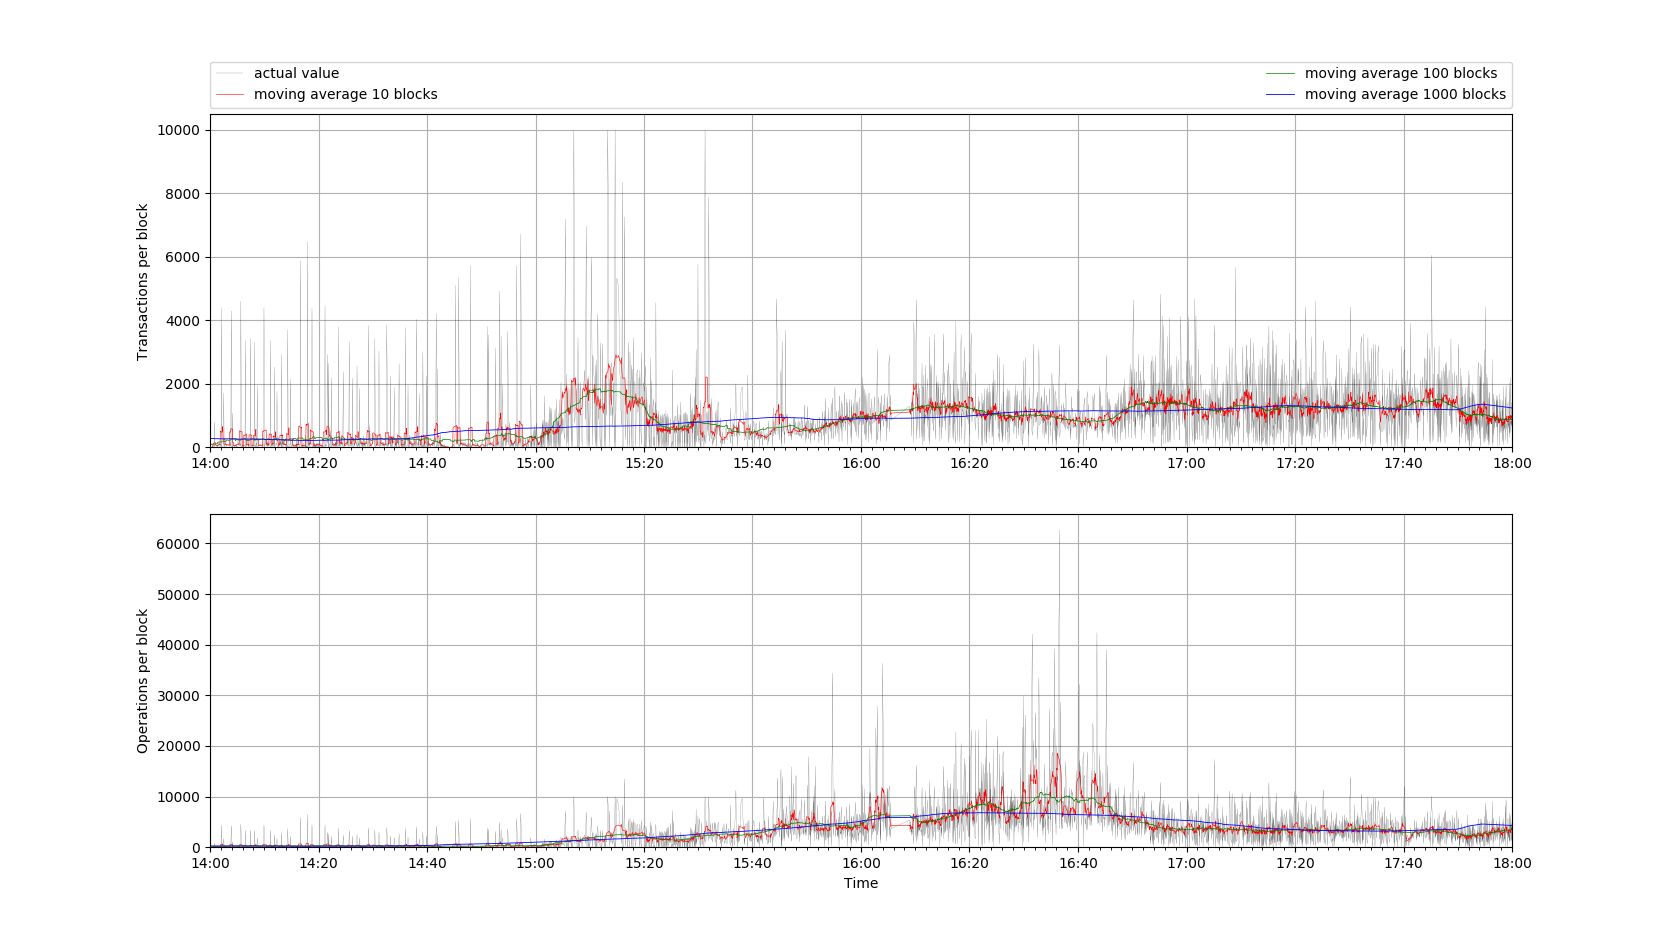
\includegraphics[width=\linewidth]{figures/stress-test-overview.png}
 \caption{Overview of the throughput ops/s and txs/s during the whole stress-test}
 \label{fig:tpsall}
\end{figure}

Most interestingly, we observed several short peaks of processed transactions and
operations during the whole stress-test. As it turned out, the reasons of those
peaks can be explained by a single participant who decided to use his
block validating node to produce transactions. By this, he skipped the
propagation of transactions through the Peer-2-Peer network which confirms to
us that the networking code represents one of the bottlenecks.

\begin{figure}[!htp]
 \centering
 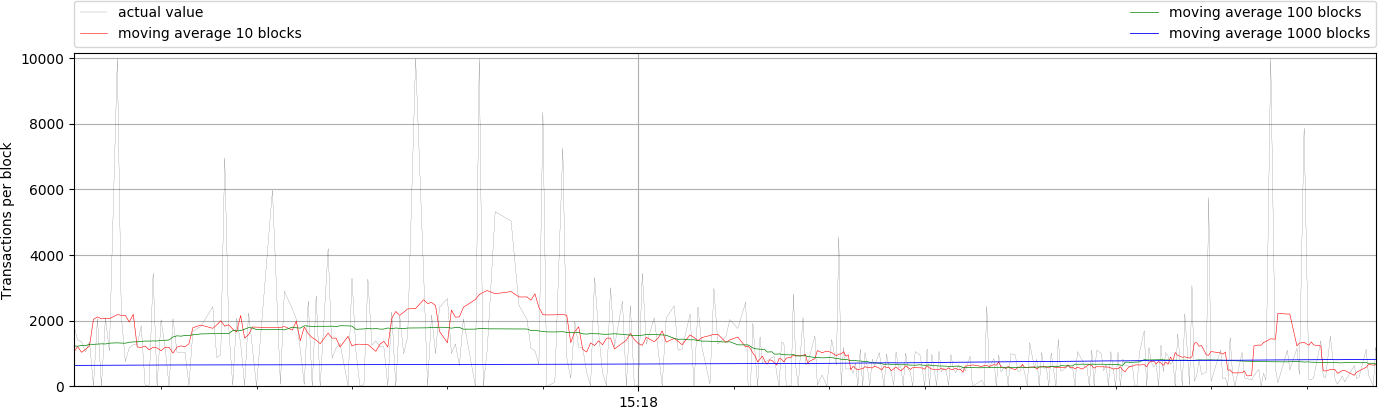
\includegraphics[width=\linewidth]{figures/stress-test-max-tps.png}
 \caption{Max ops/s during the stress-test}
 \label{fig:tps}
\end{figure}

In \cref{fig:tps}, we have zoomed into a period of rather high throughput (i.e.
\SI{2500}{transactions per block}). Here, we still see the peaks produced by
skipping the networking.

\begin{figure}[!htp]
 \centering
 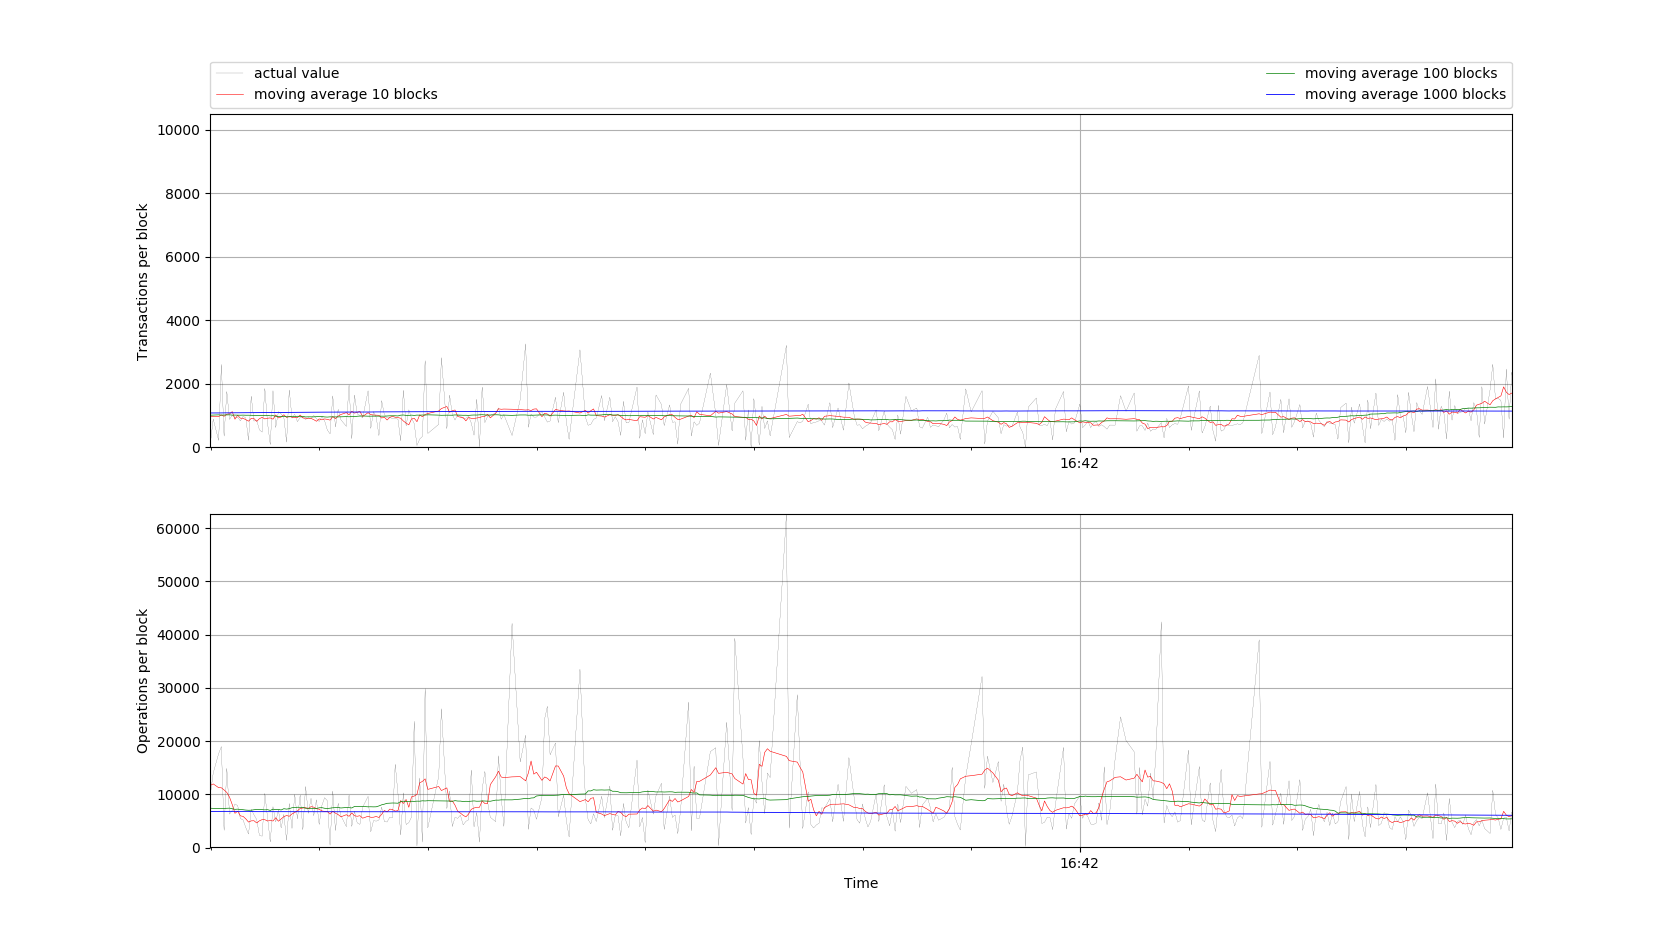
\includegraphics[width=\linewidth]{figures/stress-test-max-ops.png}
 \caption{Max ops/s during the stress-test}
 \label{fig:ops}
\end{figure}

Finally, the results in \cref{fig:ops} show that the blockchain was able to
process an average of over \SI{8000}{operations per block} with quite high
peaks and an irregular throughput per block.

\begin{figure}[!htp]
 \centering
 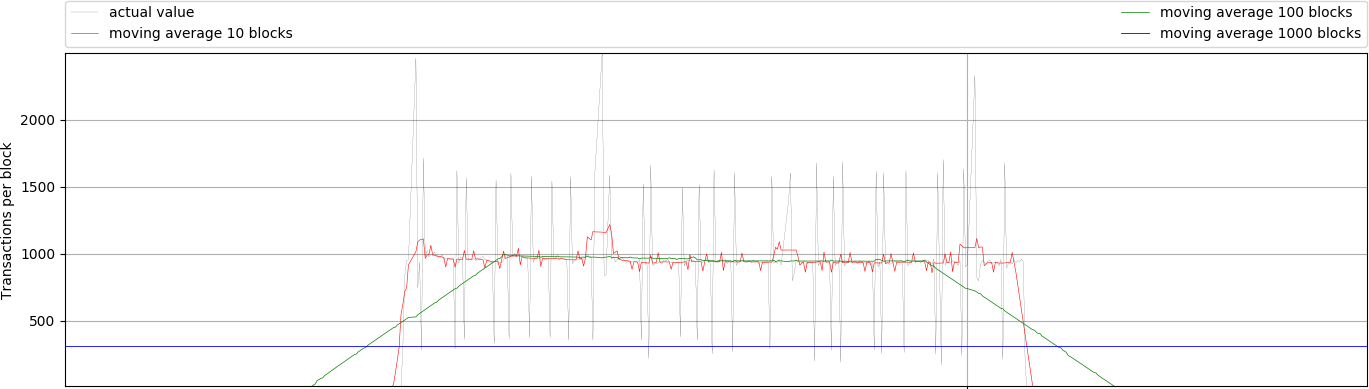
\includegraphics[width=\linewidth]{figures/stress-test-constant-load.png}
 \caption{Max ops/s during the stress-test}
 \label{fig:ops-const}
\end{figure}

The irregularity can be resolved by deploying similar hardware that can all
process the same amount of transactions/operations. We were able to confirm
this behavior later on by replacing all validators except for one, which
greatly reduces the variance of the throughput as can be seen in
\cref{fig:ops-const}. Here, the stress has been produce by a single node
connected directly to the validating node while another single validator was
only connected through the Peer-2-Peer network.
 
\subsection { Memory and Processing Requirements } \input { content/stresstest/results-hardware   } 
\section    { Conclusions                        } With our testing, we have seen that the code base is much more robust
than we had expected. The block creation and block validation is
sufficiently fast so that we can run a blockchain with synchronous block
confirmations times of \SI{1}{s} without validators dropping out too
much.

The Peer-2-Peer code seems to be working nicely but results show that it
could be one of the bottlenecks currently preventing us from going
further. The computational resources of our validators have more than
enough back-off for higher throughputs but the networking code was not
able to provide sufficient data (e.g. transactions) to raise it during
our stress-test.

We have further identified another bottleneck with respect to transaction
production. Signing transactions takes more resources and we will
prepare properly for our next stress-test. This result was confirmed in
a later private testnet where 36 cores have been activated during the
test sequentially. The result was that the blockchain easily dealt with
all of the produced transactions and the throughput increasesed
accordingly, each time additional cores have been added to transaction
production.

To conclude, the current software stack still has a few limitations and
edges that need to be optimized in order to improve scalability further,
but the foundation has been designed in such a way that it allows for
even higher throughput. Our current limitations are purely in the
implementation and networking aspects than in the software and protocol
architecture.
 
\section    { Acknoledgements                    } We would like to thank every one that has participated in the
stress-test for block validation, transaction generation and setup of a
robust Peer-2-Peer network. We would like to further acknowledge the
assistance during the preparations of the stress-test and the feedback
we have received while writing this paper. Last but not least we
appreciate the financial support given by each and everyone that has
been running a machine for the stress-test and BitShares-Munich for
providing the major API node on bitshares.eu.
 

\bibliographystyle{IEEEtran}
\bibliography{literature}
%\nocite{*}
\end{document}
